\documentclass[letterpaper]{article}
\usepackage[margin=1in]{geometry}
\usepackage[utf8]{inputenc}
\usepackage{textcomp}
\usepackage{amssymb}
\usepackage{natbib}
\usepackage{graphicx}
\usepackage{gensymb}
\usepackage{amsthm, amsmath, mathtools}
\usepackage[dvipsnames]{xcolor}
\usepackage{enumerate}
\usepackage{mdframed}
\usepackage[most]{tcolorbox}
\usepackage{csquotes}
% https://tex.stackexchange.com/questions/13506/how-to-continue-the-framed-text-box-on-multiple-pages

\tcbuselibrary{theorems}

\newcommand{\R}{\mathbb{R}}
\newcommand{\Z}{\mathbb{Z}}
\newcommand{\N}{\mathbb{N}}
\newcommand{\Q}{\mathbb{Q}}
\newcommand{\C}{\mathbb{C}}
\newcommand{\code}[1]{\texttt{#1}}
\newcommand{\mdiamond}{$\diamondsuit$}
\newcommand{\PowerSet}{\mathcal{P}}
\newcommand{\Mod}[1]{\ (\mathrm{mod}\ #1)}
\DeclareMathOperator{\lcm}{lcm}

%\newtheorem*{theorem}{Theorem}
%\newtheorem*{definition}{Definition}
%\newtheorem*{corollary}{Corollary}
%\newtheorem*{lemma}{Lemma}
\newtheorem*{proposition}{Proposition}


\newtcbtheorem[number within=section]{theorem}{Theorem}
{colback=green!5,colframe=green!35!black,fonttitle=\bfseries}{th}

\newtcbtheorem[number within=section]{definition}{Definition}
{colback=blue!5,colframe=blue!35!black,fonttitle=\bfseries}{def}

\newtcbtheorem[number within=section]{corollary}{Corollary}
{colback=yellow!5,colframe=yellow!35!black,fonttitle=\bfseries}{cor}

\newtcbtheorem[number within=section]{lemma}{Lemma}
{colback=red!5,colframe=red!35!black,fonttitle=\bfseries}{lem}

\newtcbtheorem[number within=section]{example}{Example}
{colback=white!5,colframe=white!35!black,fonttitle=\bfseries}{def}

\newtcbtheorem[number within=section]{note}{Important Note}{
        enhanced,
        sharp corners,
        attach boxed title to top left={
            xshift=-1mm,
            yshift=-5mm,
            yshifttext=-1mm
        },
        top=1.5em,
        colback=white,
        colframe=black,
        fonttitle=\bfseries,
        boxed title style={
            sharp corners,
            size=small,
            colback=red!75!black,
            colframe=red!75!black,
        } 
    }{impnote}
\usepackage[utf8]{inputenc}
\usepackage[english]{babel}
\usepackage{fancyhdr}
\usepackage[hidelinks]{hyperref}

\pagestyle{fancy}
\fancyhf{}
\rhead{CSE 131}
\chead{Monday, May 08, 2023}
\lhead{Lecture 16}
\rfoot{\thepage}

\setlength{\parindent}{0pt}

\begin{document}

\section{Structured Data: Pairs (Continued)}
In this section, we’ll discuss more about structured data, in particular pairs.

\subsection{Memory Representation}
Suppose we have the following program: 
\begin{verbatim}
    (pair 5 (pair 6 (pair 7 nil)))\end{verbatim}
The way we compile this is to first compile the left-most part of the pair (\code{5}), and then the right-most part of the pair (the rest of the pair, in this case). In particular,
\begin{itemize}
    \item The instructions for any nested expressions get evaluated before we move those values onto the heap for the current pair.
    \begin{mdframed}
        In this program's case, we evaluate \code{5} first, and then \code{6}, and then \code{7}. We put all of them on the stack first. \emph{Then}, we put 7 onto the heap first (while \code{6} and \code{5} wait). 
    \end{mdframed}
    
    \item The first pair that gets allocated is the innermost pair. 
\end{itemize}
If we assume left-to-right evaluation order, then \code{7} goes on the heap first. In this sense, allocation happens inside-out. In any case, in the heap, we expect the memory layout to look like
\begin{center}
    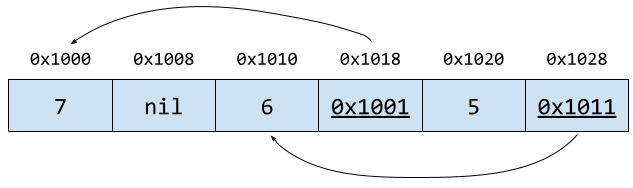
\includegraphics[scale=0.67]{../assets/pair_heap.png}
\end{center}
\textbf{Remarks:} 
\begin{itemize}
    \item We have \code{0x1001} and \code{0x1011} (instead of \code{0x1000} and \code{0x1010}) because we use \code{0x01} as the tag value for the pair.
    \item Note that, in our implementation of the compiler, we're actually going to store the integer multiplied by 2 (e.g., 14, 12, and 10, respectively), since in memory we're storing the \emph{tagged} value. In this example, we're just showing the integers as is (with no tagging).
    \item This program would evaluate to \code{0x1021}, since this is the memory address to the first element in the pair. 
\end{itemize}

\begin{mdframed}
    Another way to think about this is as follows: if we wanted to translate this program into something like Python, syntatically this would look like 
    \begin{verbatim}
        p1 = (7, nil);
        p2 = (6, p1);
        p3 = (5. p2);\end{verbatim}
    We had to \emph{allocate} memory for \code{p1} (the innermost pair), and then allocate memory for \code{p2}, and then finally for \code{p3}.
\end{mdframed}

Let's now suppose we have the following program:
\begin{verbatim}
    (fun (inc lst)
        (if (= lst nil)
            nil
            (pair (+ (fst lst) 1) (inc (snd lst)))
        )
    )

    (inc (pair 70 (pair 800 nil)))\end{verbatim}
The heap diagram might look something like 
\begin{center}
    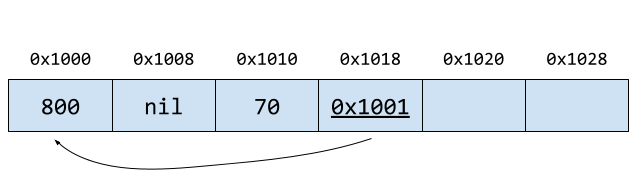
\includegraphics[scale=0.6]{../assets/pair_heap2.png}
\end{center}
Here, the result of \code{(pair 70 (pair 800 nil))} is \code{0x1011}, so \code{0x1011} is passed into the \code{inc} function. If we look at the function itself, we can see that the function itself will return the same pair, pair, nil structure.
\begin{center}
    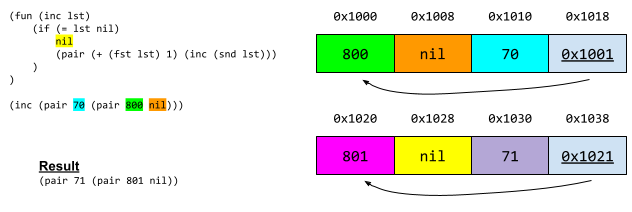
\includegraphics[scale=0.73]{../assets/pair_heap3.png}
\end{center}
And, in this exmaple. this function would return \code{0x1031}, the address to the newly created pair.

\subsection{Equality}
Let's consider the following program: 
\begin{verbatim}
    (let (point1 (pair 6 5))
        (let (point2 (pair 6 5))
            (block 
                (print (= point1 point1))                       // A
                (print (= point1 point2))                       // B
                (let (pointpair1 (pair point1 point2))
                    (let (pointpair2 (pair point1 point2))
                        (block 
                            (print (= pointpair2 pointpair2))   // C
                            (print (= pointpair1 pointpair2))   // D
                        )
                    )
                )
            )
        )
    )\end{verbatim}
We now need to decide what this program should print. More specifically, however, we need to figure out how equality of pairs will work. This introduces two types of equalities:
\begin{itemize}
    \item \textbf{Reference equality:} are the two operands referring to the same memory address? For example, in Python, this is \code{==}.
    \item \textbf{Structural equality:} are the two operands equal when considering their structures? For example, in Python, this is \code{is}.
\end{itemize}
With this in mind, we have 
\begin{center}
    \begin{tabular}{|c|c|c|}
        \hline 
        Statement & Reference Equality & Structural Equality \\ 
        \hline
        A & \code{true} & \code{true} \\ 
        B & \code{false} & \code{true} \\ 
        C & \code{true} & \code{true} \\ 
        D & \code{false} & \code{true} \\ 
        \hline  
    \end{tabular}
\end{center}
Note statements (C) and (D); if we want structural equality, we probably want to do \emph{recursive structural equality!} 

\end{document}